\section{Optical spring constant derivation}
\label{app:A} 
%\subsection{Optical spring constant}
%\label{sec:Apx1}

In this section we consider the effect of light stored in a detuned Fabry-Perot cavity using a classical approach.
The intra-cavity power generates radiation pressure that exerts on the cavity mirror a force $F_{rad}=-K_{OS}\cdot x$,
where $x$ is the mirror displacement and $K_{OS}$ is the optical spring constant.
Here we show the full derivation of the optical spring constant $K_{OS}$.

We consider a suspended Fabry-Perot cavity of length $L_0$ %shined by a laser light 
with an incident beam of wavelength $\lambda$ and power $P_0$.
First we calculate a general expression of the intra-cavity power and then its  radiation pressure force exerted on the end mirror.\\


\begin{figure}[htbp]
	\centering
		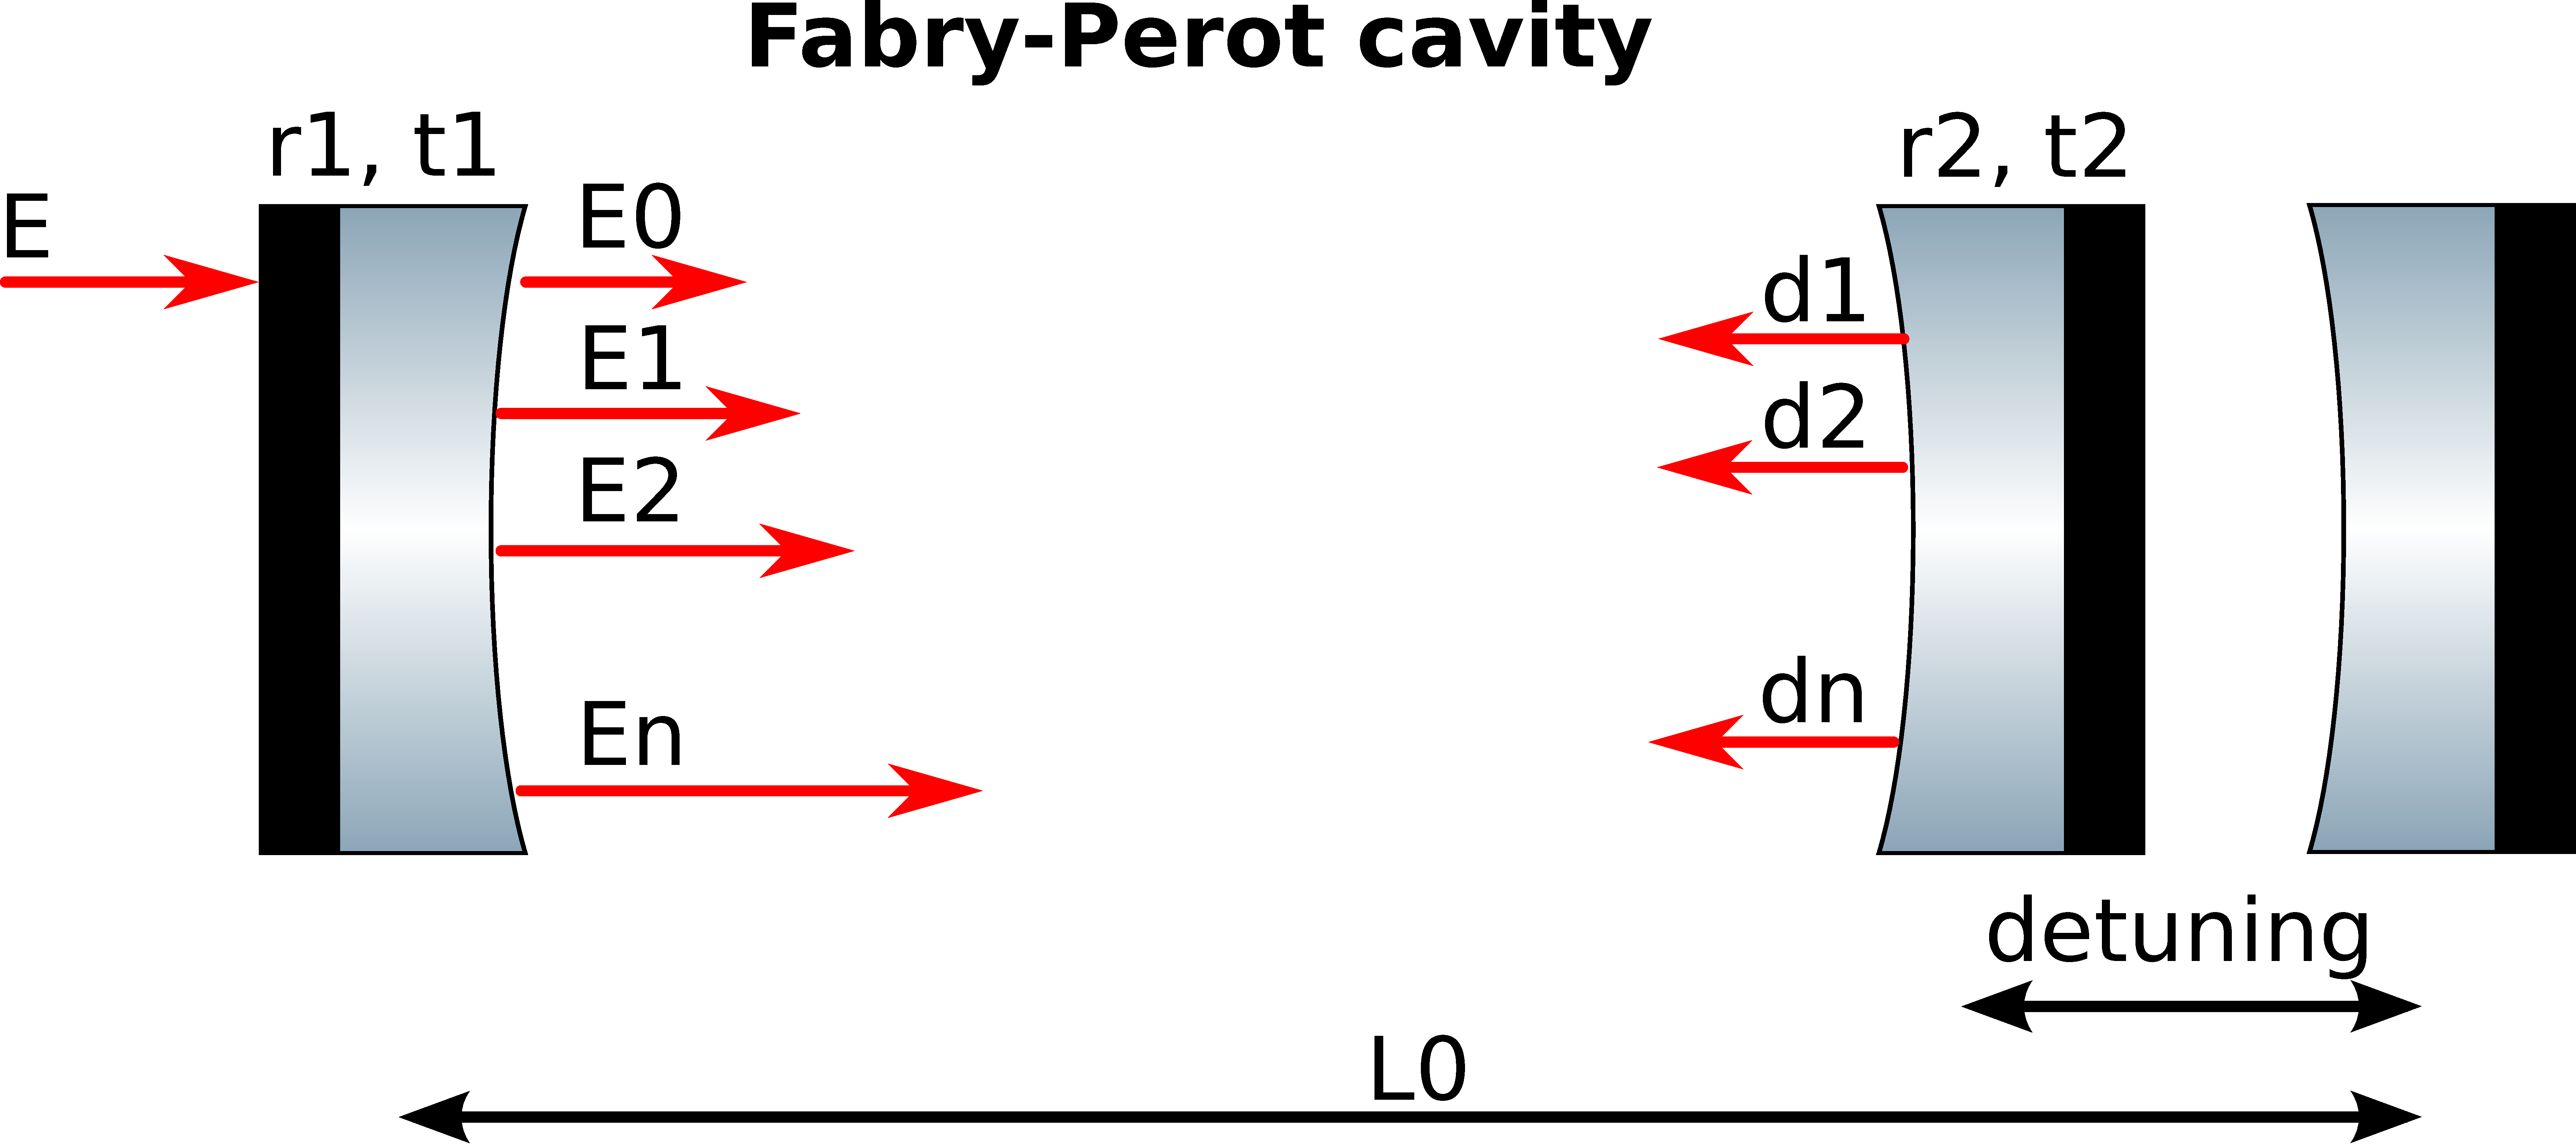
\includegraphics[width=8cm]{./images/cavity_paper.pdf}
	\caption{A Fabry-Perot cavity of length $L_0$ and coefficients $r_1,t_1$ and $r_2,t_2$ for the input and end mirrors respectively. 
	The input mirror is stationary while the end mirror is affected by harmonic motion. The incoming field $E$ at each round-trip $i$ adds up a phase shift due to the displacement $d_i$}
	\label{fig:cavity_k}
\end{figure}


The field $E=A_0e^{i\omega t}$ enters the cavity through the input mirror of coefficient $t_1=t$ and $r_1$ and the field inside the cavity at the input mirror can be seen as following

\begin{eqnarray}
E_{tot}=E_0+E_1+E_2+E_3+...+En+...
\end{eqnarray}


We consider in our model the following definitions, with $d_n$ being the displacement of the mirror,

\begin{eqnarray}
L_1&=&2(L_0+d_1)\\
L_2&=&2(2L_0+d_1+d_2)\nonumber\\
L_3&=&2(3L_0+d_1+d_2+d_3)\,\, \nonumber\\ %\mbox{with} \,\,d_n=d(t-(2n-1)\tau)\nonumber\\
...\nonumber
\end{eqnarray}
with 
\begin{eqnarray}
\label{eqn:dn1}
d_n &=& d(t-[(2n-1)\tau + \alpha_n ]) \quad \mbox{and}\\
\label{eqn:dn2}
\alpha_n &=& 2\sum\limits_{l=1}^{n-1}\frac{d_l}{c}-\frac{d_n}{c}
\end{eqnarray}

where $\tau=L_0/c$.
With the round trip length $L=2L_0$  we obtain

\begin{eqnarray}
E_{tot}&=&tE(1\!+\!r_1r_2 e^{-ikL_1}\!\!+\!(r_1r_2)^2 e^{-ikL_2}\nonumber\\
&+&(r_1r_2)^3 e^{-ikL_3}  \cdots )\nonumber\\
&=&tE(1\!+\!r_1r_2 e^{-ikL}e^{-2ikd_1}\!\!+\!(r_1r_2)^2 e^{-2ikL}e^{-2ik(d_1\!+\!d_2)}\nonumber\\
&+&(r_1r_2)^3 e^{-3ikL}e^{-2ik(d_1\!+\!d_2\!+\!d_3)}  \cdots )\nonumber
\end{eqnarray}



If we define $X=r_1r_2 e^{-ikL}$ we have 

\begin{eqnarray}
E_{tot}=tE(1+Xe^{-2ikd_1} +X^2e^{-2ik(d_1+d_2)}\nonumber\\
+X^3e^{-2ik(d_1+d_2+d_3)} \cdots )\nonumber
\end{eqnarray}

Since by definition the optical spring $K_{OS}$ is the linear term in the expansion $F=F_0+ K_{OS} d + O(d^2)$, we now expand the exponential in $d_n$. We group  $d_n$ terms:

\begin{eqnarray}
E_{tot}&=&tE(1+X(1-2ikd_1) +X^2(1-2ik(d_1+d_2))\nonumber\\
&+&X^3(1-2ik(d_1+d_2+d_3)) + \cdots )\nonumber \\
\nonumber \\
&=&tE(1+X+X^2+X^3 +\cdots\nonumber\\
&-& 2ikd_1(X+X^2+X^3\cdots)\nonumber\\
&-&2ikd_2(X^2+X^3+X^4\cdots)\nonumber\\  
&-&2ikd_3(X^3+X^4+X^5\cdots)+\cdots) \nonumber \\
\nonumber \\
%&=&tE(\frac{1}{1-X}-2ikd_1\frac{X}{1-X}-2ikd_2\frac{X^2}{1-X}\nonumber \\
%&-&2ikd_3\frac{X^3}{1-X}+\cdots) \nonumber \\
%\nonumber \\
&=&\frac{tE}{1-X}(1-2ikd_1 X-2ikd_2 X^2-2ikd_3 X^3+\cdots) \nonumber
\end{eqnarray}
Since any correction from $\alpha_n$ (equation \ref{eqn:dn2}) is quadratic in $d(t)$, we can again neglect it by definition, and find for the harmonic mirror motion (i.e. in the Fourier domain)
\begin{eqnarray}
d_n&=&x_0e^{i\Omega(t-(2n-1)\tau)}=x_0e^{i\Omega t}e^{-i\Omega(2n-1)\tau}\nonumber\\
&=&x_0e^{i\Omega t} \frac{Y^{2n}}{Y}\frac{Y}{Y}=Y^{2n-2}d_1
\end{eqnarray}

where $Y=e^{-i\Omega\tau}$. Thus we can write


\begin{eqnarray}
E_{tot}&=&\frac{tE}{1-X}(1-2ikd_1 X-2ikd_1 Y^2X^2\nonumber\\
&-&2ikd_1 Y^4 X^3-2ikd_1 Y^6 X^4\cdots)\\
&=&\frac{tE}{1-X}\nonumber\\
&\times &\left[1-2ikd_1 X(1+ Y^2X+ Y^4 X^2+Y^6 X^3\cdots)\right]\nonumber\\
&=&\frac{tE}{1-X}\left [1-\frac{2ikd_1 X}{1-Y^2X}\right ]
\end{eqnarray}

where $d_1$ is a complex number. Since we have to take its real part $Re (d_k)=\frac{d_k+\bar{d}_k}{2}$,
we consider the field inside the cavity with $\bar{d}_k$ conjugate of $d_k$:

\begin{eqnarray}
\frac{tE}{1-X}\left [1-\frac{2ik\bar{d}_1 X}{1-\overline{Y}^2 X}\right ]
\end{eqnarray}

and we obtain as total field $E$

\begin{eqnarray*}
E_{tot}=tE\left [\frac{1}{1-X}- \frac{2ikX}{2(1-X)}   \left ( \frac{d_1}{1-Y^2 X} +\frac{\bar{d}_1}{1-\overline{Y}^2 X}\right )\right]
\end{eqnarray*}

and its complex conjugate 

\begin{eqnarray*}
\overline{E}_{tot}=t\overline{E}\left [\frac{1}{1-\overline{X}}+\frac{2ik\overline{X}}{2(1-\overline{X})}   \left ( \frac{\bar{d}_1}{1-\overline{Y}^2 \overline{X}}+\frac{d_1}{1-Y^2 \overline{X}}\right )\right]
\end{eqnarray*}
 
Using the following expression
 
\begin{eqnarray}
d_1=x_0e^{i\Omega(t-\tau)}=x_0e^{i\Omega t}e^{-i\Omega\tau}=xY  
\end{eqnarray}
 
%Since we are interested only in the linear terms of $d_n$, 
%we neglect $O(d^2)$ terms (\tcb{Stefan could you write a sentence here to say "WHY"?})
we can now obtain the intra-cavity power expression by multiplying $E_{tot}$ by its conjugate
and considering only the linear terms of $x$
%(we neglect $O(d^2)$ terms \tcb{Stefan could you write a sentence here to say "WHY"?})
 
\begin{eqnarray}
P&=&E_{tot}\cdot \overline{E}_{tot}=P_0 t^2[ \frac{1}{(1-X)(1-\overline{X})}\nonumber\\  
&-&\frac{ikX xY}{(1-\overline{X})(1-X)(1-Y^2 X)} -
\frac{ikX \bar{x}\overline{Y}}{(1-\overline{X})(1-X)(1-\overline{Y}^2 X)}\nonumber \\
&+&\frac{ik\overline{X} \bar{x}\overline{Y} } {(1-\overline{X})(1-X)(1-\overline{Y}^2 \overline{X})}+ 
\frac{ik\overline{X} xY}{(1-\overline{X})(1-X)(1-Y^2 \overline{X})}]  \nonumber \\
%\frac{k^2 |X|^2}{4(1-X)(1-\overline{X})} \left( 
%\frac{|x|^2|Y|^2}{(1-Y^2 X)(1-\overline{Y}^2\overline{X})}+
%\frac{|x|^2|Y|^2}{(1-\overline{Y}^2 X)(1-Y^2\overline{X}) }+\nonumber 
%\frac{x^2 Y^2}{(1-Y^2 X)(1-Y^2\overline{X})}+
%\frac{\bar{x}^2 \bar{Y}^2}{(1-\overline{Y}^2 X)(1-\overline{Y}^2\overline{X})}
%\right) ]   
 %\right] 
\end{eqnarray}

where we have also neglected the first constant term. We now group the terms in $x$ and $\bar{x}$:

\newpage
\begin{eqnarray}
%\centering
P&=&-P_0t^2 [ \frac{ikY}{(1-\overline{X})(1-X)} \left( \frac{X}{1-Y^2 X}-\frac{\overline{X}}{1-Y^2\overline{X}} \right) x\nonumber\\
&+&\frac{ik\overline{Y}}{(1-\overline{X})(1-X)} \left( \frac{X}{1-\overline{Y}^2 X}-\frac{\overline{X}}{1-\overline{Y}^2\overline{X}} \right)\bar{x} ]=\nonumber \\
&=&-P_0t^2 [ \frac{ikY}{(1-\overline{X})(1-X)}\nonumber\\ 
&\times &\left( \frac{X}{1-Y^2 X}-\frac{\overline{X}}{1-Y^2\overline{X}} \right) x + cc ]
\end{eqnarray}

Once we have calculated the power we can obtain the radiation pressure force on the end mirror by $F_{rad}=\frac{2 r_2^2}{c}P$. Furthermore
we can also notice the similarity of the expression with the elastic force. Thus we recall that
in frequency domain and complex notation $K$ is defined by $F=-Kx$, the real form is thus

\begin{eqnarray*}
F'=Re[F]=-\frac{1}{2}(Kx+\overline{K}\bar{x})=-\frac{1}{2}(Kx+cc)
\end{eqnarray*}

Taking into account that we are calculating the radiation pressure on the end mirror, we need to consider an extra delay factor $Y$
for the calculation of the power which appears in the expression of $K$. The complex spring is then given by 

\begin{eqnarray*}
%\centering
K=\frac{2 r_2^2}{c} P_0 t^2  \frac{2ikY^2}{(1-\overline{X})(1-X)} \left( \frac{X}{1-Y^2 X}-\frac{\overline{X}}{1-Y^2\overline{X}} \right) 
\end{eqnarray*}
which can be rewritten in the form of equations \ref{KOS_full_2}
and \ref{eqn:K0}.


\subsection*{Detuning}
Given the frequency detuning is $\delta=\omega_0-\omega_{res}$ and $\Omega=\omega-\omega_0$,
where $\omega_0$ is the carrier (sub-carrier) frequency and $\omega_{res}$ is the resonant frequency, we get the following expressions:

\begin{eqnarray}
\mbox{\textit{Resonance}}\nonumber\\ 
\lambda_{res}&=& L/n, \quad k_{res}=\frac{2\pi n}{L}, \nonumber\\ 
\omega_{res} & = & k_{res}\cdot c = \frac{2\pi n}{L} \cdot c\\
\mbox{\textit{Carrier}}\nonumber\\ 
\lambda_0 & = &\lambda,  \quad k_0=\frac{2\pi}{\lambda}=k, \nonumber\\ 
\omega_0 & = & k_0\cdot c=\frac{2\pi c}{\lambda}=w_{res}+\delta\\
\mbox{\textit{Sideband}}\nonumber\\
\omega &=& \Omega+\omega_0=\Omega+\delta+\omega_{res}
\end{eqnarray}

Thus we find
\newpage
\begin{eqnarray}
e^{-ikL}\equiv e^{-ik_0L}=e^{-i\omega_0 \frac{L}{c}}\nonumber\\
=e^{-i(\omega_{res}+\delta)\frac{L}{c}}=e^{-i\omega_{res}\frac{L}{c}}e^{-i\delta\frac{L}{c}}
\end{eqnarray}
Recalling that $\tau=\frac{L_0}{c}=\frac{L}{2c}$ we can write
\begin{eqnarray}
e^{-ikL}=e^{-i\delta 2\tau}%\approx 1-i\delta 2\tau
\end{eqnarray}

%For a negative  detuning
%\begin{eqnarray}
%e^{-ikL} &=& e^{-i(\omega_{res}-\delta)\frac{L}{c}}\nonumber\\
%&=&e^{-i\omega_{res}\frac{L}{c}}e^{i\delta\frac{L}{c}}% \approx 1+i\tau2\delta
%\end{eqnarray}

If we now replace $X$ and $Y$ we obtain the exact expression for $K$:%the most general expression of $K$ that has seen so far 

\begin{eqnarray}
%\centering
K_{OS}=&-P_0 t^2 r_2^2 \frac{4ike^{-2i\Omega\tau}}{c(1-r_1\!r_2e^{i2\delta\tau})(1-r_1\!r_2e^{-i2\delta\tau})}\times\nonumber\\
 & \left( \frac{r_1\!r_2e^{-i\delta \tau}}{1\!-\!r_1\!r_2e^{-2i\Omega\tau} e^{-i2\delta\tau}}
 \!-\!\frac{r_1\!r_2e^{i2\delta\tau}}{1\!-\!r_1\!r_2e^{-2i\Omega\tau}e^{i2\delta\tau}} \right) 
\end{eqnarray}


To compare to existing literature we now expand the exponentials to linear order 
in $\Omega$ and $\delta$, 
$e^{-i\delta 2\tau}\approx 1-i\delta 2\tau$
and $e^{-i2\Omega \tau}\approx 1-i2\Omega \tau$:

\begin{eqnarray}
K =& -P_0 t^2 r_2^2 \times \nonumber\\
& \frac{4ik(1-2i\Omega\tau)r_1r_2}{c(1-r_1r_2+r_1r_2i2\delta\tau)(1-r_1r_2-r_1r_2i2\delta\tau)}\times\\
& \left[\frac{1-i2\delta\tau}{1-r_1r_2(1-2i\Omega\tau-i2\delta\tau)} -\frac{1+i2\delta\tau}{1-r_1r_2(1-2i\Omega\tau+i2\delta\tau)} \right] \nonumber 
\end{eqnarray}

%\begin{eqnarray}
%=-P_0 t^2 r_2^2 \times\nonumber \\
%\frac{4ik(1-2i\Omega\tau)r_1r_2}{c(1+\frac{r_1r_2}{1-r_1r_2}i2\delta\tau)(1-\frac{r_1r_2}{1-r_1r_2}i2\delta\tau)(1-r_1r_2)^3}\nonumber\\
%\left[\frac{1-i\tau2\delta}{1+\frac{r_1r_2}{1-r_1r_2}2i\Omega\tau+\frac{r_1r_2}{1-r_1r_2}i2\delta\tau} -
%\frac{1+i\tau2\delta}{1+\frac{r_1r_2}{1-r_1r_2}2i\Omega\tau-\frac{r_1r_2}{1-r_1r_2}i2\delta\tau}
%\right]\nonumber
%\end{eqnarray}

Considering the $Finesse \approx \pi \frac{r_1r_2}{1-r_1r_2}= \pi FSR/\gamma$, the cavity bandwidth $\gamma$, and the free spectral range $FSR=1/2\tau$, we obtain:

\begin{eqnarray}
K_{OS}\approx-P_0 t^2 r_2^2 \frac{4ik(1-2i\Omega\tau)r_1r_2}{c(1+i\frac{\delta}{\gamma})(1-i\frac{\delta}{\gamma})(1-r_1r_2)^3} \nonumber\\
\times\left[\frac{1-i2\delta}{1+\frac{\Omega}{\gamma}i+\frac{\delta}{\gamma}i} -
\frac{1+i2\delta}{1+\frac{\Omega}{\gamma}i-\frac{\delta}{\gamma}i}
\right]
\end{eqnarray}

Finally, since they correspond to a simple time delay, we neglect the $i\Omega\tau$, $i\delta\tau$ terms in the numerator and obtain
\begin{eqnarray}
K_{OS} & \approx & P_0 t^2 r_2^2 \frac{8k r_1r_2}{c(1-r_1r_2)^3}\frac{ \frac{\delta}{\gamma}}{(1+\frac{\delta^2}{\gamma^2})} 
\left[\frac{1}{1+\frac{\delta^2}{\gamma^2}-\frac{\Omega^2}{\gamma^2}+i2\frac{\Omega}{\gamma} }\right]\nonumber\\
%& = & \frac{K_0}{1+\frac{\delta^2}{\gamma^2}-\frac{\Omega^2}{\gamma^2}+i2\frac{\Omega}{\gamma}}
\end{eqnarray}

\subsubsection{Overcoupled cavity}

In the particular case of perfectly over-coupled cavity ($r_2=1$) $Finesse/\pi=2/T_1$ and $(1-r_1r_2)^2=T_1^2/2$ and the optical spring constant becomes:

\begin{eqnarray}
K_{OS} & \approx & 128 P_0  \frac{\pi}{c\lambda T_1^2}\frac{ \frac{\delta}{\gamma}}{(1+\frac{\delta^2}{\gamma^2})} 
\left[\frac{1}{1+\frac{\delta^2}{\gamma^2}-\frac{\Omega^2}{\gamma^2}+i2\frac{\Omega}{\gamma} }\right]\nonumber\\
\label{eqn:overcoupled}
%& = & \frac{K_0}{1+\frac{\delta^2}{\gamma^2}-\frac{\Omega^2}{\gamma^2}+i2\frac{\Omega}{\gamma}}
\end{eqnarray}

\subsubsection{Matched cavity}

In this case of a matched cavity ($r_1=r_2$) $Finesse/\pi=1/T_1$ and $(1-r_1r_2)^2=T_1^2$ and the optical spring constant remains the same as in Eq.\,\ref{eqn:overcoupled} except for the the factor 128 which has to be replaced with 16.



\section{Torsion pendulum mechanical plant}
\label{app:B} 

Here we transform
the basis of coordinates $\{x_G,\Theta\}$  formed by the position of the center of gravity $x_G$ of the mirror and its rotation angle $\Theta$  with respect to the vertical axis passing from $x_G$ into a basis $\{x_A,x_B\}$ formed by the length of the cavities relative to beam A and beam B respectively. Thus the longitudinal and angular control of the mirror can be treated as the longitudinal control of the two above mentioned cavities. The basis can be expressed as
%
%\begin{eqnarray}
%\label{base}
%x_A = x_G +r_A\Theta \\ \nonumber
%x_B = x_G + r_B\Theta
%\end{eqnarray}

\begin{equation}
\label{eqn:BDEF}
\begin{pmatrix}
x_A \\ x_B
\end{pmatrix}
=
 \begin{pmatrix}
1& r_A\\1& r_B
\end{pmatrix} 
\begin{pmatrix}
x_G\\ \Theta
\end{pmatrix}
=
\mathcal{B}
\begin{pmatrix}
x_G\\ \Theta
\end{pmatrix}
\end{equation}

with $r_A$ and $r_B$ being the lever arms of the two beams with respect to $x_G$.

The equation of motion for the mirror is
\begin{equation}
\label{eqn:motion_matrix}
-\omega^2
\begin{pmatrix}
m &  \\ & I
\end{pmatrix}
 \begin{pmatrix}
x_G\\ \Theta
\end{pmatrix}
= 
\begin{pmatrix}
F_{tot}\\ T_{tot}
\end{pmatrix}
\end{equation}
with $I$ being the moment of inertia of the mirror of mass $m$. We now express the total force and the total torque exerted on the mirror
as function of the individual forces $F_A$ and $F_B$:

\begin{equation}
\label{eqn:FtotTtot}
\begin{pmatrix}
F_{tot} \\ T_{tot}
\end{pmatrix}
=
 \begin{pmatrix}
1& 1\\r_A& r_B
\end{pmatrix} 
\begin{pmatrix}
F_A\\ F_B
\end{pmatrix}
=
\mathcal{B}^{T}
\begin{pmatrix}
F_A\\ F_B
\end{pmatrix}
\end{equation}

Using equations \ref{eqn:FtotTtot} and \ref{eqn:BDEF} in equation \ref{eqn:motion_matrix} we obtain the equation of motion in the ${x_A,x_B}$ basis:
\begin{equation}
-\omega^2
\left[
\mathcal{B}^{T-1}
\begin{pmatrix}
m &  \\ & I
\end{pmatrix}
\mathcal{B}^{-1}
\right ]
 \begin{pmatrix}
x_A\\ x_B
\end{pmatrix} 
=
\begin{pmatrix}
F_{A}\\ F_{B}
\end{pmatrix}
\end{equation}

\section{Stability in two dimensions}
\label{app:C}
The control loop stability in multiple dimensions can be evaluated by considering the one-dimensional open-loop transfer function of every control filter (i.e. optical spring) while all other loops stays closed. Here we calculate these open-loop transfer functions for the two-dimesnional case.

Refering to figure \ref{fig:block_loops}, we inject a signal $F_{xa}=F_{\rm ext}$ into port A. The output at port A is $F_{ya}=F_A$. We close the loop from output B to input B by feeding back the force $F_B$.
%We inject an external signal $n=F_{xa}-F_{ya}$ along the loop A  %as it could be a swept-sine from a network analyser
%to measure the open loop transfer function for cavity A. %while beam B loop remain closed. That can be represented as:
%\begin{equation}
%HM
%\left( \begin{array}{c}
%F_A\\F_B
%\end{array} \right)
%+
%HM
%\left( \begin{array}{c}
%n\\0
%\end{array} \right)
%=
%\left( \begin{array}{c}
%F_{A}\\F_B
%\end{array} \right)
%\end{equation}
%with $n$ being an external signal injected between $F_{xa}$ and $F_{ya}$. %as in practice could
%be a swept-sine injected from a network analyser. 
%Inserting $n=F_{xa}-F_{ya}$ and 
We obtain the following expression:
\begin{equation}
HM
\left( \begin{array}{c}
0\\F_B
\end{array} \right)
+
HM
\left( \begin{array}{c}
F_{xa}\\0
\end{array} \right)
=
\left( \begin{array}{c}
F_{ya}\\F_B
\end{array} \right)
\end{equation}
If we introduce the $2\times2$ matrix $S$: 
\begin{equation}
S_A=
\left( \begin{array}{cc}
0 & 0\\
0 & 1
\end{array} \right)
\end{equation}
we can  write
\begin{equation}
HMS_A
\left( \begin{array}{c}
F_{ya}\\F_B
\end{array} \right)
+
HM
\left( \begin{array}{c}
F_{xa}\\0
\end{array} \right)
=
\left( \begin{array}{c}
F_{ya}\\F_B
\end{array} \right)
\end{equation}
Using the vector $e_A^{T}=(1,0)$ we are able to extract the following open loop
transfer function related to cavity A:
\begin{equation}
OL_{A}=\frac{F_{ya}}{F_{xa}}=e_A^{T}(\mathbb{I}-HMS_A)^{-1}HMe_A
\end{equation}

The same open loop transfer function can be obtained considering an external signal injected into the loop of the beam B while the loop of beam A remains closed.

\begin{equation}
OL_{B}=\frac{F_{yb}}{F_{xb}}=e_B^{T}(\mathbb{I}-HMS_B)^{-1}HMe_B
\end{equation}

with $e_B^{T}=(0,1)$ and % $S_B$:

\begin{equation}
S_B=
\left( \begin{array}{cc}
1 & 0\\
0 & 0
\end{array} \right)
\end{equation}


